\input{preamble}
\usepackage{graphicx}

% Title
\begin{document}
\begin{singlespace}
\title{First Results}
\author{Austyn West\thanks{Department of Economics, Texas A\&M University.}}
\date{November 20, 2025}
\maketitle
\end{singlespace}

\section*{Descriptive Statistics}


\begin{table}[htbp]
\centering
\caption{Summary Statistics for E-Rate Funding Requests}
\label{tab:erate_summary_stats}
\begin{threeparttable}
\begin{tabular}{ l c c c c }
\toprule
& \textbf{Mean} & \textbf{Std. Dev.} & \textbf{25th pct.} & \textbf{75th pct.} \\
& (1) & (2) & (3) & (4) \\
\midrule
\multicolumn{5}{l}{\underline{\textbf{Panel a. Financial Amounts}}} \\ \\
\hspace{2mm} \textbf{\textit{Requested Invoice Amount}} & 11,902 & 90,203 & 480 & 4,580 \\
\hspace{2mm} \textbf{\textit{Approved Invoice Amount}} & 10,081 & 74,060 & 275.230 & 3,868 \\
\hspace{2mm} \textbf{\textit{Log Requested Amount}} & 7.310 & 2.083 & 6.186 & 8.431 \\
\hspace{2mm} \textbf{\textit{Discount Rate}} & 70.644 & 20.355 & 60 & 85 \\ \\
\\ \\
\multicolumn{5}{l}{\underline{\textbf{Panel b. Flags and Status}}} \\
\hspace{2mm} \textbf{\textit{Funded Flag}} & 0.918 & 0.274 & & \\
\hspace{2mm} \textbf{\textit{Negative Requested Amount Flag}} & 0.003 & 0.056 & & \\
\hspace{2mm} \textbf{\textit{Reimbursement Flag}} & 0.097 & 0.295 & & \\
\hspace{2mm} \textbf{\textit{Funded with Comment}} & 0.017 & 0.128 & & \\
\bottomrule
\end{tabular}
\footnotesize
\textit{Notes:} This table reports summary statistics for E-Rate funding requests submitted by public school districts in Texas. Amount Requested refers to the total pre-discount funding amount submitted on Form 471. Approved Amount is the total amount approved for reimbursement. Log Total Amount is the natural logarithm of the requested amount after removing zero or negative values. Discount Rate is the applicant's E-Rate discount percentage based on the percentage of students on the National School Lunch Program in the district. Binary indicator variables are defined as follows: Funded Flag equals 1 if any portion of the request was approved; Negative Amount Flag equals 1 for filings with nonpositive or invalid pre-discount amounts; Reimbursement Flag equals 1 if the request includes a reimbursement decision code; and Funded with Comment equals 1 for requests that were both funded and accompanied by a reimbursement decision code. Percentile columns reflect the empirical 25th and 75th percentiles of each distribution.
\end{threeparttable}
\end{table}


Table~\ref{tab:erate_summary_stats} presents summary statistics for E-Rate funding requests submitted by Texas public school districts. Panel~A reports continuous financial measures, including requested amounts, approved amounts, and discount rates, while Panel~B summarizes binary indicators of application status.

In Panel~A, the distribution of requested amounts exhibits substantial right-skewness. The mean request is \$11,902, but the 75th percentile is only \$4,580, indicating that the mean is heavily influenced by a small number of large requests. This skewness motivates the use of logarithmic transformations in subsequent analyses, where the log requested amount has a more symmetric distribution with mean 7.31 (SD 2.08). The substantial right-skewness of the requested amounts is visually confirmed in Figure~\ref{fig:log_density}, which plots the density of the natural logarithm of requested amounts. While the raw dollar amounts are heavily skewed, the log-transformed variable approximates a symmetric, bell-shaped distribution, validating the use of logarithmic transformations in our multivariate analyses. This transformation helps mitigate the influence of extreme outliers and meets the distributional assumptions of standard regression techniques.

Approved amounts follow a similar pattern, with mean \$10,081 (SD \$74,060), suggesting modest adjustments during the review process. The discount rate distribution shows meaningful variation across districts, ranging from 60\% at the 25th percentile to 85\% at the 75th percentile around a mean of 70.6\%, reflecting the program's design where discounts are tied to the percentage of students eligible for the National School Lunch Program.

Panel~B reveals that most funding requests are successful, with 91.8\% receiving at least partial approval. Only 0.3\% of requests have nonpositive amounts, suggesting high data quality. The reimbursement flag (9.7\%) and funded with comment flag (1.7\%) indicate that while most applications are processed routinely, a nontrivial minority require additional administrative review.

\begin{figure}[h!]
    \centering
    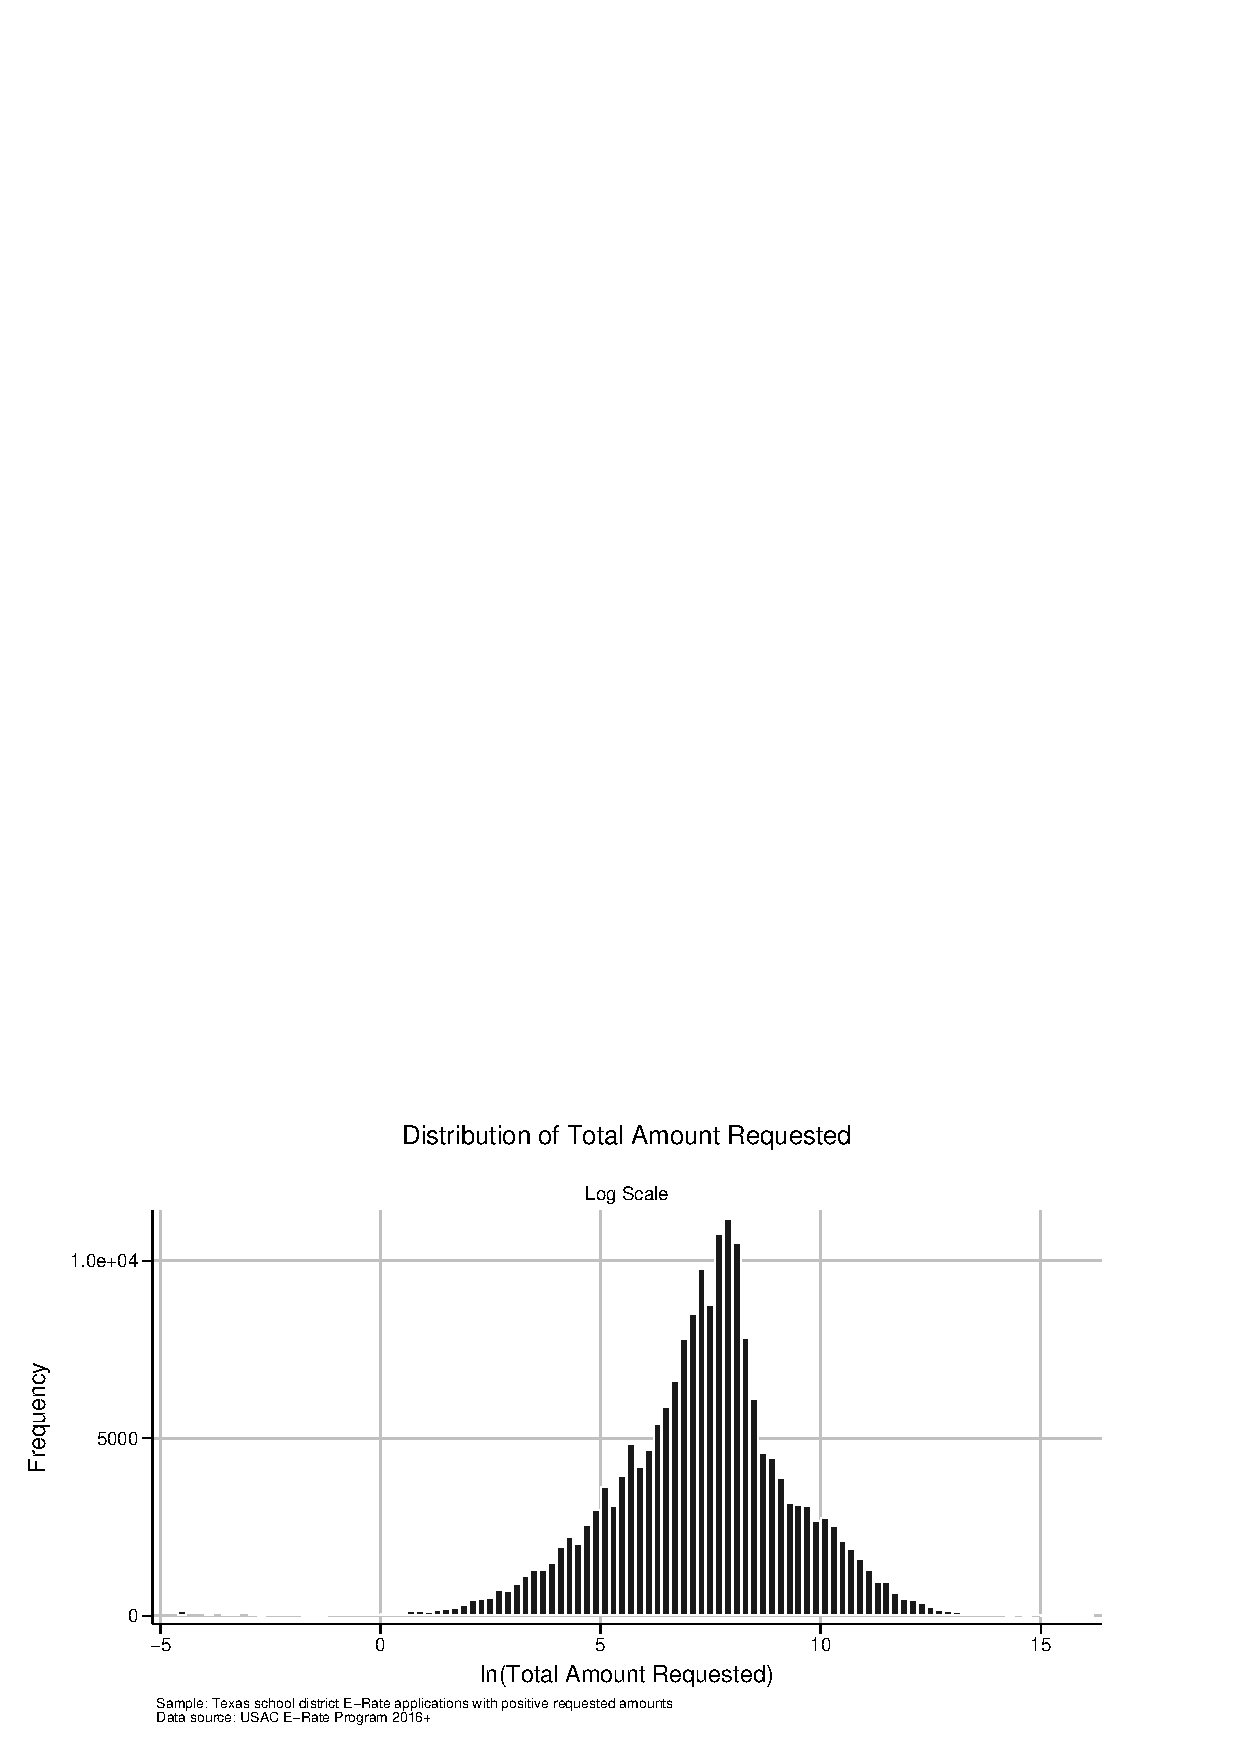
\includegraphics[width=0.8\linewidth]{Log_Amount_Requested_Density.pdf}
    \caption{Distribution of the Log-Transformed Total Amount Requested}
    \label{fig:log_density}
    \begin{minipage}{0.8\linewidth}
        \footnotesize
        \textit{Note:} This figure displays the frequency distribution of the natural logarithm of total funding amounts requested by Texas school districts in their E-Rate applications. The distribution is approximately normal, centered around a log value of 5-10, with a positive skew indicating a minority of applications requested substantially larger amounts. The log transformation reveals the underlying shape of the data, which would be heavily right-skewed in its original dollar-scale form.
    \end{minipage}
\end{figure}


These summary statistics reflect the underlying economics and administration of the E-Rate program. The heavy-tailed distribution of requested amounts likely stems from the large fixed costs associated with network infrastructure, which generates a few very large requests from districts undertaking major upgrades, alongside many smaller requests for recurring services. The high approval rate is consistent with the program's goal of universal service support, where applications are pre-screened for eligibility, and the detailed discount matrix reduces ambiguity in funding levels. The variation in discount rates directly mirrors the socioeconomic disparities between districts, as it is mechanically determined by the percentage of students eligible for free or reduced-price lunches.

These patterns have several implications for our empirical strategy. First, the heavy-tailed distribution of financial amounts suggests that median regressions (quantile regression) or parametric models using logarithmic transformations may be more appropriate than linear models using levels. Second, the high approval rate limits useful variation for studying a binary approval outcome, shifting focus to the continuous variation in approval amounts as a primary dependent variable. Third, the systematic variation in discount rates, which is quasi-exogenous as it is tied to a district's socioeconomic profile, provides a potential instrumental variable or a source of conditional randomness for identifying causal effects. The descriptive evidence thus supports modeling approaches that account for the program's institutional features and the distributional characteristics of the key variables.

\end{document}
